\section{Region Identification}\label{section:regions}

Visual breakdowns of the types of regions identified and their counts
for each \textit{Trichoderma} assembly are shown in Figure
~\ref{fig:regions-sankey}. We will discuss the types of regions,
beginning with fully supported regions. These regions, labelled `Full
Support', are sections of genomic sequence where all three gene
finders agree that a gene is present in some form. These fully
supported regions are then broken down into two categories, based on
whether the models from each gene finder agree on the start
and/or stop positions of the gene model. Regions that have support
from more than one gene finder, but not all, are labelled regions with
`Partial Support'. These regions are also broken down in to two
subtypes based on whether the gene predictions agree on the
start and/or stop positions of the gene. Regions with support from
only one gene finder are labelled as singletons.

\begin{figure}
  \centering
  \begin{subfigure}{0.9\textwidth}
    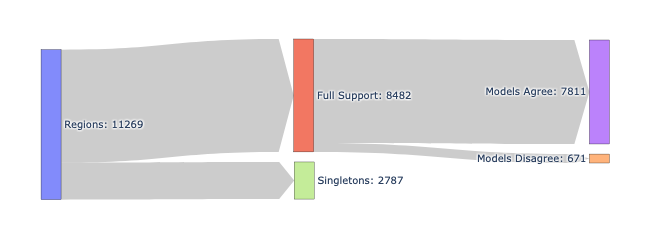
\includegraphics[width=\textwidth]{figures/dc1-region-breakdown.png}\label{fig:dc1-regions}
    \caption{DC1}
  \end{subfigure}
  \begin{subfigure}{0.9\textwidth}
    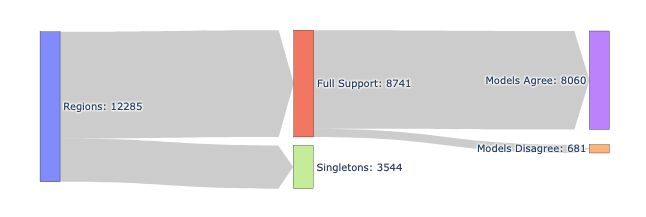
\includegraphics[width=\textwidth]{figures/tsth20-region-breakdown.png}\label{fig:tsth20-regions}
    \caption{Tsth20}
  \end{subfigure}
  \begin{subfigure}{0.9\textwidth}
    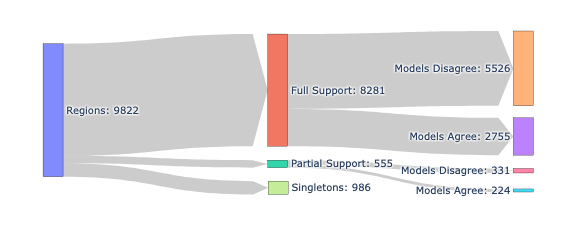
\includegraphics[width=\textwidth]{figures/t-reesei-region-breakdown.png}\label{fig:t-reesei-regions}
    \caption{\textit{T. reesei}}
  \end{subfigure}
\end{figure}
\begin{figure}
  \ContinuedFloat
  \centering
  \begin{subfigure}{0.9\textwidth}
    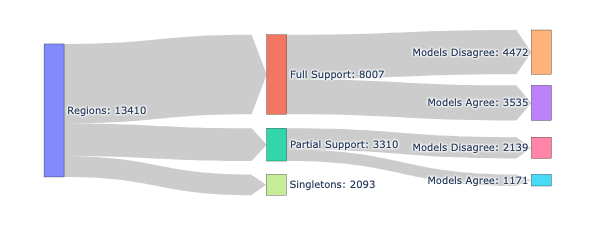
\includegraphics[width=\textwidth]{figures/t-harzianum-region-breakdown.png}\label{fig:t-harzianum-regions}
    \caption{\textit{T. harzianum}}
  \end{subfigure}
  \begin{subfigure}{0.9\textwidth}
    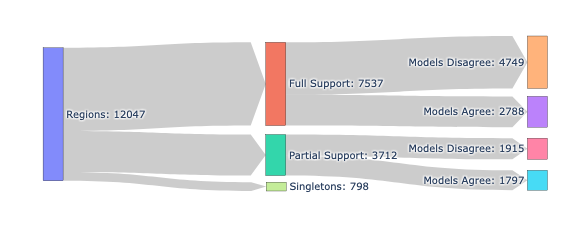
\includegraphics[width=\textwidth]{figures/t-virens-region-breakdown.png}\label{fig:t-virens-regions}
    \caption{\textit{T. virens}}
  \end{subfigure}
  \caption[Breakdown of identified regions]{Figures showing breakdowns
    of genomic regions identified by the region finding
    process. Regions, in blue, are categorized based on support from
    gene finders. Regions with supporting predictions from all gene
    finders included in this analysis are labelled with `Full Support'
    and colored red. Fully supported regions are then broken down into
    regions where gene models agree on the start and stop positions of
    the genes (purple), and those that do not (orange). Regions
    labelled with `Partial Support' (turquoise) are regions with
    supporting gene predictions from two gene finders. Partially
    supported regions are also broken down into regions in which gene
    finders agree on the start and stop positions of the gene (cyan),
    and those that do not agree (pink). Regions with gene predictions
    from only one gene finder are labelled as singletons (green).}\label{fig:regions-sankey}
\end{figure}

Looking at DC1 and Tsth20 in Figure~\ref{fig:regions-sankey}, it
appears that Braker2 and GeneMark predict genes in the same regions in
the 69\% and 65\% of cases, respectively. For regions with full
support in DC1 and Tsth20, the models also tend to agree on the start
and stop positions of the gene in that region. This is not generally
the case as we will see later when RefSeq is also considered. There
are no regions with partial support for DC1 and Tsth20, as there are
only two gene finders considered. \textit{Trichoderma reesei} contains
the fewest number of regions, which seems to scale appropriately with
the total number of predicted genes and assembly length. Eighty-four
percent of the regions are fully or partially supported by Braker2,
GeneMark and RefSeq, with only 10 percent of the regions being single
tool predictions. The most interesting observation here is the extent
to which fully supported regions disagree on start and stop positions
of the gene(s) in each region. There is clearly a difference in the
gene models being produced by these gene finders. If there is also
more disagreement on the start and stop positions of a gene, then
there is likely disagreement on the number and location of exons and
introns within the gene model as well. In the case of partially
supported regions, there is roughly 50\% to 60\% agreement on start
and stop positions, but that may come as less of a surprise as there
is already disagreement on presence by definition. Gene finding
behavior in regions from \textit{T.harzianum} and \textit{T. virens}
differ from the other assemblies in the split between fully and
partially supported regions. There seems to be fewer regions with full
support from all gene finders and the reason why is unclear. The gene
models in each region, whether fully or partially supported, still
tend to disagree on start and stop positions of the genes more often
than agree.

It is also worthwhile investigating some potentially interesting cases
of strange gene calls in regions. One such case is when a region
contains more than three individual predicted genes. The null
hypothesis, so to speak, is that if all gene finders agree exactly on
the presence and position of a gene in a region, then one should
expect exactly three predictions in that region. We observe that this
is not always true. Cases of more than three gene predictions in a
region were present in regions from all processed assemblies. Figure
~\ref{fig:uncertain-regions} shows an example of one of these regions,
in which the single gene predicted by RefSeq spans multiple gene
predictions from both Braker2 and GeneMark. In the case of DC1 and
Tsth20, there were very few regions that matched this scenario, with
19 and 6 regions containing more than 3 gene predictions,
respectively. Conversely, \textit{T. reesei, T.harzianum and T.virens}
contain many such regions, with assemblies reporting 546, 899 and 521
regions with greater than three gene predictions, respectively. While
having predictions from each gene finding tool present in a region is
a strong indicator for the presence of a gene, having more than one
gene prediction per gene finder raises questions about which model (or
models) is correct and why disagreement exists.

\begin{figure}
  \centering
  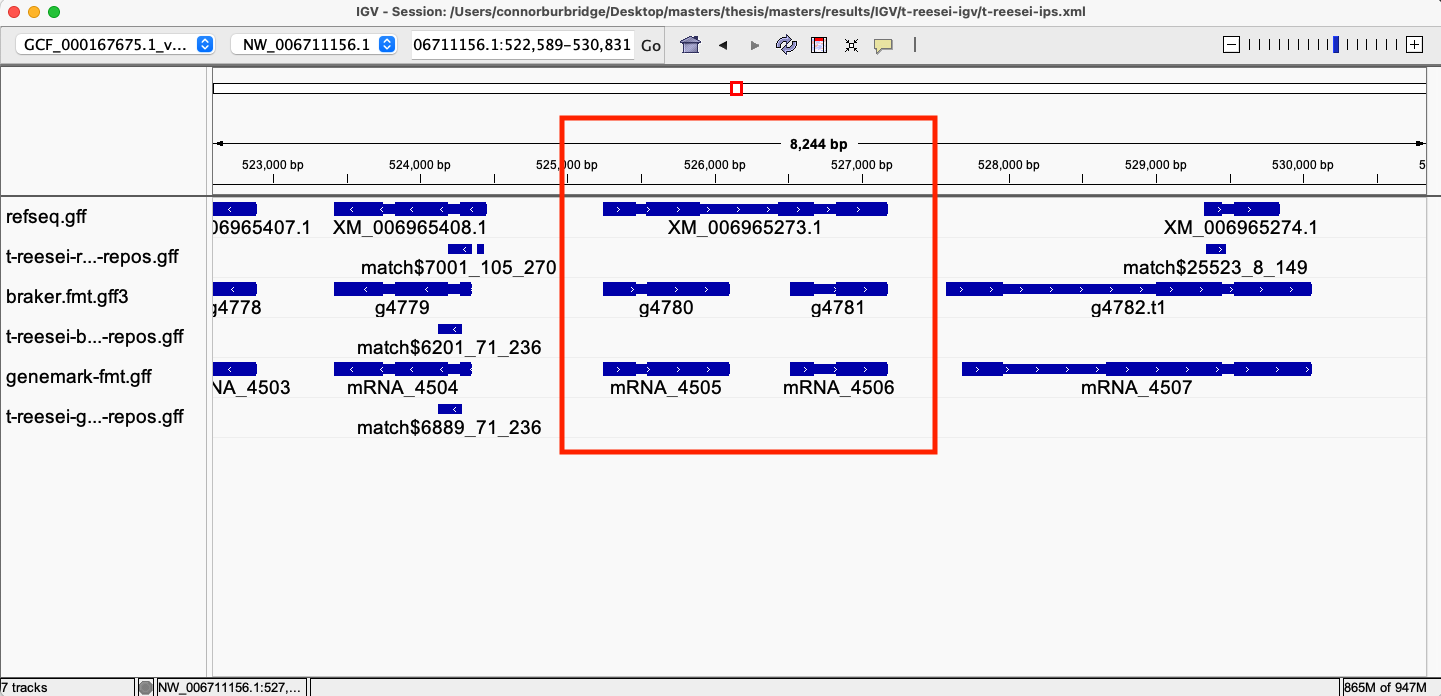
\includegraphics[width=0.9\textwidth]{figures/igv/igv-uncertain-regions.png}
  \caption[Example of a region with many gene calls]{An IGV screenshot
    from \textit{T. reesei} showing a region containing five gene
    predictions in which one of the gene finders disagrees with the
    other two, highlighted in the red box.}\label{fig:uncertain-regions}
\end{figure}

Another interesting set of criteria to investigate is whether
gene finders always predict genes on the same strand within a
region. We observe that regions containing predictions on different
strands do exist, and are observed in predictions from all assemblies
included in this analysis. Figure~\ref{fig:opposing-strands} shows an
example of a region containing gene predictions on opposing
strands. As in the case of regions with more than three gene
predictions, DC1 and Tsth20 have fewer mixed strand regions with 29
regions identified in DC1 and 46 regions identified in Tsth20. Results
from \textit{T. reesei, T. harzianum} and \textit{T. virens} show more
regions in which this property is true, with region counts of 203, 533
and 293 respectively. Under the assumption that gene finders should
predict the same genes on the same strands, it is unexpected to find
so many of these cases, although it is possible that these overlapping
sense and anti-sense genes exist naturally~\cite{wright2022a}.

\begin{figure}
  \centering
  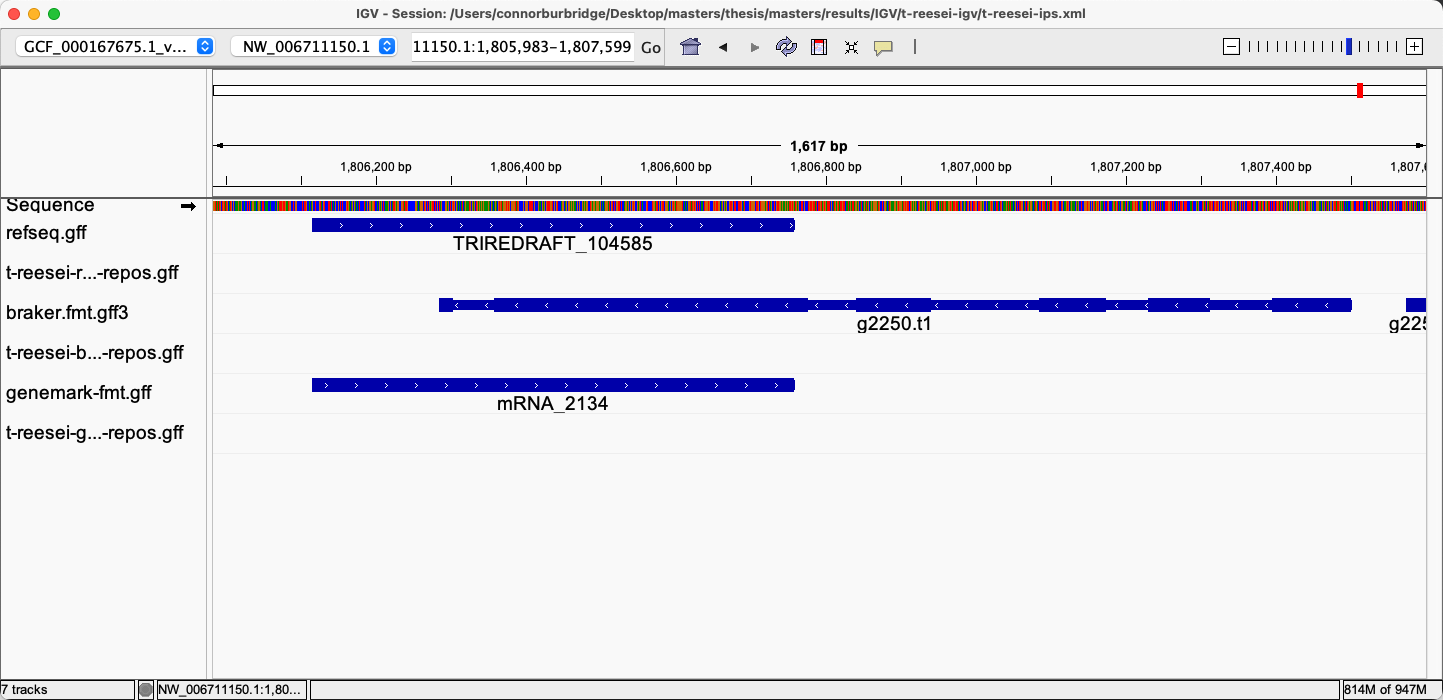
\includegraphics[width=0.9\textwidth]{figures/igv/igv-opposing-strands.png}
  \caption[Predictions on opposing strands]{An IGV screenshot of
    \textit{T. reesei} showing a region which contains gene
    predictions on opposite strands.}\label{fig:opposing-strands}
\end{figure}

In summary, gene finders agree partially or completely on the presence
of a gene in the vast majority of cases. While gene finders generally
agree on the presence of a gene, they tend to disagree on the
underlying gene model more often than they agree, except in the
case of DC1 and Tsth20. This is likely due to only including two gene
finders in their analysis rather than three, resulting in fewer
opportunities for disagreement. This observation is true when applied
to the start and stop positions of the gene, but further investigation
and comparison of intronic and exonic sequences between genes may
provide more insight. It is also possible that genome quality may
affect agreement between gene finders as the underlying model may be
trained on contigs that are larger or of different structure than the
assembly it is applied to. This is particularly true in the cases of
DC1 and Tsth20, which are composed of larger contigs in comparison to
the assemblies from NCBI. Finally, regions identified in this analysis
do not always fit the ideal scenario of one gene prediction from each
tool per region. Regions in which there are more than three gene
predictions were observed in all assemblies included in this work. In
addition, we observe cases where gene finders predict genes on
different strands.
